\documentclass{beamer}
\usepackage[T1]{fontenc}
\usepackage[utf8]{inputenc}

\usetheme{Madrid}
\usecolortheme{default}
\usepackage{amsmath,amssymb,amsfonts,amsthm}
\usepackage{mathtools}
\usepackage{txfonts}
\usepackage{tkz-euclide}
\usepackage{listings}
\usepackage{adjustbox}
\usepackage{array}
\usepackage{gensymb}
\usepackage{multicol}
\usepackage{gensymb}
\usepackage{tabularx}
\usepackage{gvv}
\usepackage{lmodern}
\usepackage{circuitikz}
\usepackage{tikz}
\lstset{literate={·}{{$\cdot$}}1 {λ}{{$\lambda$}}1 {→}{{$\to$}}1}
\usepackage{graphicx}

\setbeamertemplate{page number in head/foot}[totalframenumber]

\usepackage{tcolorbox}
\tcbuselibrary{minted,breakable,xparse,skins}



\definecolor{bg}{gray}{0.95}
\DeclareTCBListing{mintedbox}{O{}m!O{}}{%
  breakable=true,
  listing engine=minted,
  listing only,
  minted language=#2,
  minted style=default,
  minted options={%
    linenos,
    gobble=0,
    breaklines=true,
    breakafter=,,
    fontsize=\small,
    numbersep=8pt,
    #1},
  boxsep=0pt,
  left skip=0pt,
  right skip=0pt,
  left=25pt,
  right=0pt,
  top=3pt,
  bottom=3pt,
  arc=5pt,
  leftrule=0pt,
  rightrule=0pt,
  bottomrule=2pt,
  toprule=2pt,
  colback=bg,
  colframe=orange!70,
  enhanced,
  overlay={%
    \begin{tcbclipinterior}
    \fill[orange!20!white] (frame.south west) rectangle ([xshift=20pt]frame.north west);
    \end{tcbclipinterior}},
  #3,
}
\lstset{
    language=C,
    basicstyle=\ttfamily\small,
    keywordstyle=\color{blue},
    stringstyle=\color{orange},
    commentstyle=\color{green!60!black},
    numbers=left,
    numberstyle=\tiny\color{gray},
    breaklines=true,
    showstringspaces=false,
}
\title{7.4.17}
\subtitle{Circle equation}
\author{EE25BTECH11010 - Arsh Dhoke}
\date{}
\begin{document}

\frame{\titlepage}

\begin{frame}{Question}
If the lines $2x + 3y + 1 = 0$ and $3x - y - 4 = 0$ lie along the diameter of a circle of circumference $10\pi$, then the equation of the circle is:

\begin{multicols}{2}
\begin{enumerate}
\item $x^2 + y^2 + 2x - 2y - 23 = 0$
\item $x^2 + y^2 - 2x - 2y - 23 = 0$
\item $x^2 + y^2 + 2x + 2y - 23 = 0$
\item $x^2 + y^2 - 2x + 2y - 23 = 0$
\end{enumerate}
\end{multicols}
\end{frame}

\begin{frame}{Equation of Circle}
\begin{align}
\vec{x}^{T}\vec{V}\vec{x} + 2\vec{u}^{T}\vec{x} + f = 0
\end{align}
where $\vec{V}$ is an identity matrix of order 2.
\begin{align}
2x + 3y + 1 = 0, \quad 3x - y - 4 = 0
\end{align}
\end{frame}

\begin{frame}{Finding Intersection (Centre)}
\begin{align}
\myvec{2 & 3 \\ 3 & -1}\vec{x} = \myvec{-1 \\ 4}
\end{align}
Augmented form:
\begin{align}
\augvec{2}{2}{2 & 3 & -1 \\ 3 & -1 & 4}
\end{align}
Performing row operations:
\begin{align}
\augvec{2}{2}{2 & 3 & -1 \\ 3 & -1 & 4}
&\xrightarrow[R_2 \to R_2 - \frac{3}{2}R_1]{}
\augvec{2}{2}{2 & 3 & -1 \\ 0 & -\frac{11}{2} & \frac{11}{2}} \\
&\xrightarrow[R_2 \to \frac{2}{-11}R_2]{}
\augvec{2}{2}{2 & 3 & -1 \\ 0 & 1 & -1} \\
&\xrightarrow[R_1 \to R_1 - 3R_2]{}
\augvec{2}{2}{2 & 0 & 2 \\ 0 & 1 & -1} 
\end{align}
\end{frame}

\begin{frame}{Centre and Radius}
\begin{align}
&\xrightarrow[R_1 \to \frac{1}{2}R_1]{}
\augvec{2}{2}{1 & 0 & 1 \\ 0 & 1 & -1} \\
\vec{x} &= \myvec{1 \\ -1} \\
\Rightarrow \vec{c} &= \myvec{1 \\ -1}
\end{align}
Given circumference $10\pi \Rightarrow r = 5 \Rightarrow r^2 = 25.$
\end{frame}

\begin{frame}{Finding Constants}
\begin{align}
\vec{V} &= \vec{I}, \quad \vec{c} = -\vec{u} \\
\Rightarrow \vec{u} &= -\myvec{1 \\ -1} = \myvec{-1 \\ 1} \\
f &= \vec{c}^{T}\vec{V}\vec{c} - r^2 = 2 - 25 = -23
\end{align}
\end{frame}

\begin{frame}{Final Equation of Circle}
\begin{align}
(\vec{x})^{T}\vec{I}\vec{x}+ 2\myvec{-1 & 1}\vec{x}- 23 &= 0 \\
(\vec{x})^{T}\vec{x}+ 2\myvec{-1 & 1}\vec{x}- 23 &= 0
\end{align}
Substituting $\vec{x}=\myvec{x \\ y}$,
\begin{align}
x^2 + y^2 - 2x + 2y - 23 = 0
\end{align}
\end{frame}

\begin{frame}{Graphical Representation}
\begin{figure}[ht!]
\centering
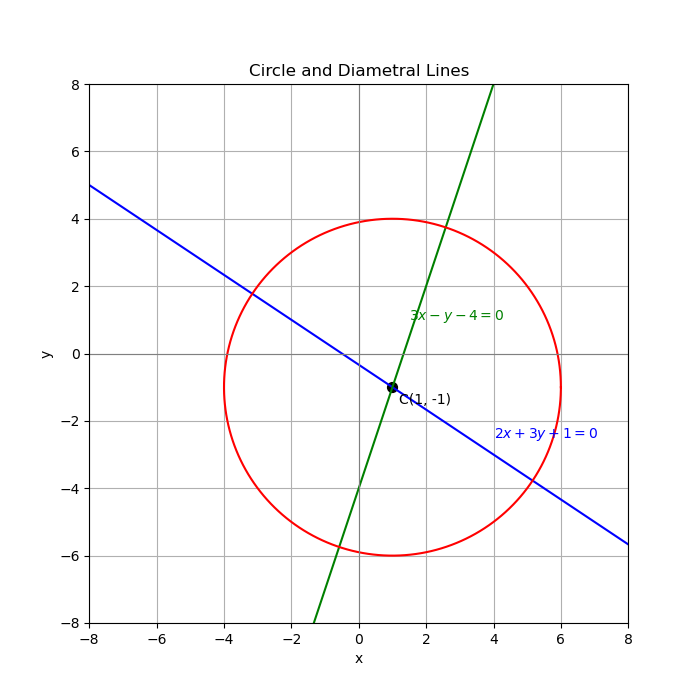
\includegraphics[width=0.7\textwidth]{figs/circle.png}
\caption{Graph showing the circle and diametral lines}
\end{figure}
\end{frame}

\begin{frame}[fragile]
    \frametitle{C Code}
\begin{lstlisting}
#include <math.h>

// Function to solve circle given two lines on diameter and circumference
void circle_from_diameter_lines(double a1, double b1, double c1,
                                double a2, double b2, double c2,
                                double circumference,
                                double coeffs[5]) {
    // Find intersection point of the two lines (midpoint of diameter)
    double det = a1*b2 - a2*b1;
    double x0 = (b1*c2 - b2*c1)/det;
    double y0 = (a2*c1 - a1*c2)/det;

    // Radius from circumference: 2*pi*r = circumference
    double r = circumference / (2*M_PI);
    double r2 = r*r;
\end{lstlisting}
\end{frame}

\begin{frame}[fragile]
    \frametitle{C Code}
\begin{lstlisting}
    // Circle equation: (x - x0)^2 + (y - y0)^2 = r^2
    // Expand: x^2 + y^2 - 2*x0*x - 2*y0*y + (x0^2 + y0^2 - r^2) = 0
    coeffs[0] = -2*x0;                    // D
    coeffs[1] = -2*y0;                    // E
    coeffs[2] = x0*x0 + y0*y0 - r2;      // F
    coeffs[3] = 1.0;                      // Coefficient of x^2
    coeffs[4] = 1.0;                      // Coefficient of y^2
}
\end{lstlisting}
\end{frame}

\begin{frame}[fragile]
    \frametitle{Python Code}
\begin{lstlisting}
import numpy as np
import matplotlib.pyplot as plt

# Circle parameters
h, k = 1, -1
r = 5

# Line equations
x = np.linspace(-8, 8, 400)
y1 = (-2*x - 1)/3          # 2x + 3y + 1 = 0
y2 = 3*x - 4               # 3x - y - 4 = 0

# Circle
theta = np.linspace(0, 2*np.pi, 400)
xc = h + r * np.cos(theta)
yc = k + r * np.sin(theta)

# Plot setup
plt.figure(figsize=(7,7))
\end{lstlisting}
\end{frame}

\begin{frame}[fragile]
    \frametitle{Python Code}
\begin{lstlisting}
plt.plot(x, y1, color='blue')
plt.plot(x, y2, color='green')
plt.plot(xc, yc, color='red')

# Centre
plt.scatter(h, k, color='black', s=50)
plt.text(h+0.2, k-0.5, 'C(1, -1)', fontsize=10)

# Annotate equations beside lines 
# For 2x + 3y + 1 = 0
plt.text(4, (-2*4 - 1)/3 + 0.5, r'$2x + 3y + 1 = 0$', color='blue', fontsize=10)

# For 3x - y - 4 = 0
plt.text(1.5, 3*(1.5) - 4 + 0.5, r'$3x - y - 4 = 0$', color='green', fontsize=10)
\end{lstlisting}
\end{frame}

\begin{frame}[fragile]
    \frametitle{Python Code}
\begin{lstlisting}
# Axes and styling
plt.axhline(0, color='gray', linewidth=0.8)
plt.axvline(0, color='gray', linewidth=0.8)
plt.gca().set_aspect('equal', adjustable='box')

plt.xlim(-8, 8)
plt.ylim(-8, 8)
plt.xlabel('x')
plt.ylabel('y')
plt.title('Circle and Diametral Lines')
plt.grid(True)
plt.savefig("/home/arsh-dhoke/ee1030-2025/ee25btech11010/matgeo/7.4.17/figs/circle.png")
plt.show()

\end{lstlisting}
\end{frame}


\begin{frame}[fragile]
    \frametitle{Python+ C Code}
\begin{lstlisting}
import ctypes
import numpy as np
import matplotlib.pyplot as plt

# Load the shared library
lib = ctypes.CDLL('./code.so')

# Define argument and return types
lib.circle_from_diameter_lines.argtypes = [
    ctypes.c_double, ctypes.c_double, ctypes.c_double,  # line1 a,b,c
    ctypes.c_double, ctypes.c_double, ctypes.c_double,  # line2 a,b,c
    ctypes.c_double,                                    # circumference
    ctypes.POINTER(ctypes.c_double)                     # coeffs array
]
lib.circle_from_diameter_lines.restype = None
\end{lstlisting}
\end{frame}

\begin{frame}[fragile]
    \frametitle{Python+ C Code}
\begin{lstlisting}
# Prepare coefficients array
coeffs = (ctypes.c_double * 5)()

# Call the function: example lines 2x+3y+1=0, 3x-y-4=0, circumference=10*pi
lib.circle_from_diameter_lines(2, 3, 1, 3, -1, -4, 10*3.141592653589793, coeffs)

coeffs_list = list(coeffs)
print("Circle coefficients [D, E, F, x^2 coeff, y^2 coeff]:", coeffs_list)

# Extract center and radius
D, E, F, _, _ = coeffs_list
x0 = -D/2
y0 = -E/2
r = np.sqrt(x0**2 + y0**2 - F)
\end{lstlisting}
\end{frame}

\begin{frame}[fragile]
    \frametitle{Python+ C Code}
\begin{lstlisting}
# Plot the circle
theta = np.linspace(0, 2*np.pi, 500)
x = x0 + r*np.cos(theta)
y = y0 + r*np.sin(theta)

plt.figure(figsize=(6,6))
plt.plot(x, y, label='Circle')
plt.scatter([x0], [y0], color='red', label='Center')
plt.gca().set_aspect('equal', 'box')
plt.title('Circle from two diameter lines')
plt.xlabel('x')
plt.ylabel('y')
plt.grid(True)
plt.legend()
plt.savefig("/home/arsh-dhoke/ee1030-2025/ee25btech11010/matgeo/7.4.17/figs/circle.png")
plt.show()

\end{lstlisting}
\end{frame}
\end{document}
